\chapter{Teorema de \emph{Noether}. Rotaciones}

	
\begin{tikzpicture}
	\fill [left color=red!50, right color=teal!50] (0,0) rectangle (6.5,.1);
	\fill [left color=teal!50, right color=blue!50] (6.5,0) rectangle (11.5,.1);
	\end{tikzpicture}


\vspace{10mm}
\begin{adjustwidth}{50pt}{50pt}
\begin{ejemplo}

En este tema estudiaremos las rotaciones y como expresarlas como una transformación infinitesimal. Veremos que para lagrangianos de potencial central e invariantes con el tiempo, la acción es invariante frente a rotaciones y que la carga conservada en este caso (Noether) es el momento angular.

\end{ejemplo}
\end{adjustwidth}
\vspace{-5mm}

\section {Teorema de \emph{Noether}. Rotaciones}

\subsection{Otra forma de expresar el producto vectorial}
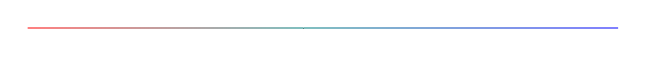
\begin{tikzpicture}
	\fill [left color=red!50, right color=teal!50] (0,0) rectangle (3.5,.01);
	\fill [left color=teal!50, right color=blue!50] (3.5,0) rectangle (7.5,.01);
	\end{tikzpicture}
\vspace{5mm}

Como vimos en el capítulo \ref{T7PotenGener} (Potencial generalizado), hay una regla mnemotécnica para recordar las componentes del producto vectorial,

$\vec a\times \vec b=\vec c \ \to \ 
\begin{cases}
\ c_1=a_2b_3-a_3b_2 \\ \  c_2=a_3b_1-a_1b_3 \\  \ c_3=a_1b_2-a_2b_1 	
\end{cases} \qquad \text{orden: } 1231231\cdots \ ,\ $ 

después del 1 va el 2, después el 3, luego el 1 de nuevo y así. Para la componente 3 del producto vectorial, por ejemplo, después de 3 vuelve el 1 y el 2, por eso aparece $a_1b_2$ y luego, restando, al revés, $a_2b_1$.


\subrayado{$\textbf{!`Truco!}$}: $\quad \vec a \times \vec b = \mqty(0& \cdots & \cdots \\ \cdots & 0 & \cdots \\ \cdots & \cdots& 0) \mqty(b_1\\b_2\\b_3) = \mqty(a_2b_3-a_3b_2\\a_3b_1-a_1b_3\\a_1b_2-a_2b_1)$

Obviamente, en la diagonal de la matriz deben haber $0$ ya que en la primera fila de la matriz resultado no hay $b_1$, ni en la segunda $b_2$, ni $b_3$ en la tercera. Razonando, obtenemos

$\vec a \times \vec b \ = \ \mqty(0& \textcolor{red}{-a_3} & \textcolor{red}{a_2} \\ \textcolor{blue}{a_3} & 0 & \textcolor{blue}{-a_1} \\ \textcolor{olive}{-a_2} & \textcolor{olive}{a_1} & 0) \ \mqty(b_1\\b_2\\b_3) \ = \  \mqty(\textcolor{red}{a_2}b_3\textcolor{red}{-a_3}b_2\\ \textcolor{blue}{a_3}b_1\textcolor{blue}{-a_1}b_3\\ \textcolor{olive}{a_1}b_2\textcolor{olive}{-a_2}b_1)$

Matriz que también podemos expresar así:

$\vec a \times \vec b \ = \ a_1 \ \mqty(0&0&0\\0&0&-1\\0&1&0) 
\ + \ a_2 \ \mqty(0&0&1\\0&0&0\\-1&0&0) \ + \ a_3 \ \mqty(0&-1&0\\1&0&0\\0&0&0)$

\begin{equation}
G_1 \ = \ \mqty(0&0&0\\0&0&-1\\0&1&0) \qquad
G_2 \ = \ \mqty(0&0&1\\0&0&0\\-1&0&0) \qquad
G_3 \ = \ \mqty(0&-1&0\\1&0&0\\0&0&0) \qquad
\overrightarrow G=(G_1.G_2,G_3)	
\end{equation}

Con lo que $\quad a_1G_1+a_2G_2+a_3G_3=\mqty(0&-a_3&a_2\\a_3&0&-a_1\\-a_2&a_1&0) = \vec a \cdot \overrightarrow G\, , \ $  es una matriz.

\vspace{5mm} 
Finalmente,

\begin{equation}
\label{T16OFEPV}
\boxed{ \ \boldsymbol{
\vec a \times \vec b \ = \ (\vec a \cdot \overrightarrow G) \cdot \vec b
} \ }	
\end{equation}


!`Ojo!, $\ \vec a \cdot \overrightarrow G\ $ es una \underline{matriz}.

\vspace{5mm}
\textbf{Propiedad de las matrices G}: $\quad \boldsymbol{G_i^T=-G_i}\, , \  i=1,2,3\ $, son \textbf{antisimétricas}.

En el siguiente apartado vamos a ver que estas matrices tienen que ver con las rotaciones.

\vspace{5mm}
\subsection{Rotaciones}
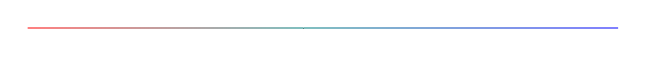
\begin{tikzpicture}
	\fill [left color=red!50, right color=teal!50] (0,0) rectangle (3.5,.01);
	\fill [left color=teal!50, right color=blue!50] (3.5,0) rectangle (7.5,.01);
	\end{tikzpicture}
\vspace{5mm}

\begin{multicols}{2}
	\begin{figure}[H]
	\centering
	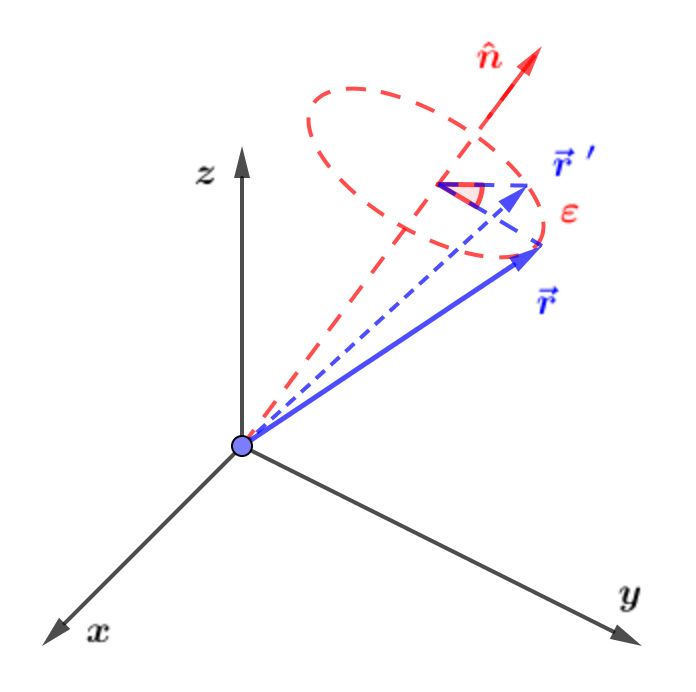
\includegraphics[width=.35\textwidth]{imagenes/img16-01.png}
\end{figure}
Rotación del vector $\vec r$, de ángulo $\theta$, alrededor del eje de vector unitario $\hat n:\quad \boldsymbol{R(\theta,\hat n)}$

Si no giramos, $\ R(0,\hat n)=I=\mqty(\imat{2})$

Una rotación de un ángulo infinitesimal $\varepsilon$, en torno al eje $\hat n$, será, aproximadamente:

 $R(\varepsilon, \hat n)\approx I+\varepsilon\cdot M$ \begin{footnotesize} (no sabemos nada del valor de $M$) \end{footnotesize}
 
 Al rotar $\vec r$ un ángulo $\theta$ alrededor de $\hat n$ obtendremos $\vec r\ ':\quad R(\theta , \hat n) \ \vec r = \vec r\ ' $

\end{multicols}

Obviamente, el módulo del vector se ha de conservar en la rotación: 

$|\vec r| = |\vec r\ '|\  \ \to \ \vec r \cdot \vec r=\vec r\ ' \cdot \vec r\ '=(R\vec r) \cdot (R\vec r)\, . \quad $
Como $\ \vec a \cdot \vec b= \mqty(a_1&a_2&a_3) \cdot \mqty(b_1 \\ b_2 \\ b_3)={\vec a}^{\ T} \cdot \vec b\, ,$

$\vec r \cdot \vec r = {\vec r}^{\ T} \cdot \vec r=\vec r\ ' \cdot \vec r\ ' ={\vec r\ '}^{\ T} \cdot \vec r \ '= 
(R\vec r\ ')^T \cdot (R\vec r)\, . \  \quad$ \begin{small}Es sabido que $\ (AB)^T=B^tA^T\, ,$ por lo que	\end{small}

$\vec r\cdot \vec r=\vec r^{\ T}\ R^T\ R\ \vec r \quad \to \quad \boldsymbol{R^TR=I}\, ,\ \ $ $\boldsymbol{R}$ \textbf{es ortogonal}. \textcolor{gris}{$\quad (R^{-1}=R^T)$}

\vspace{5mm}
$[R(\theta, \hat n)]^T \cdot R(\theta, \hat n) =I\, , \ \forall \theta \quad \to \quad $ para ángulos pequeños $\ \varepsilon<<1\, \ \varepsilon^2 \approx 0\,$:

$[I+\varepsilon M ]^T(I+\varepsilon M )\approx I  \ \to \ 
(I+\varepsilon M^T)(I+\varepsilon M)\approx I \ \to \ 
I+\varepsilon M + \varepsilon M^T +	\cancelto{0}{\mathcal{O}(\varepsilon^2)}\approx I$

Luego, $\ \cancelto{\neq 0}{\varepsilon} \ (M+M^T) = 0 \ \to \ M+M^T=0 \ \to \ \subrayado{\boldsymbol{\boxed{ \ M^T \ = \ - M \ } }}\, .\  $ Las matrices $\boldsymbol{M}$ también han de ser \textbf{antisimétricas}, como las matrices $G_i$.

\begin{myalertblock}{Rotaciones infinitesimales}
$$\boldsymbol{ R(\varepsilon ,\hat n) \ = \ I + \ \varepsilon M \ / \ M^T=-M} $$	
\end{myalertblock}

\vspace{5mm}
Una matriz antisimétrica de orden 3 tiene 3 grados de libertad,  $\ a_1,\ a_2, \ a_3 \, \ $ de modo que  

$M=\mqty(0&-a_3&a_2\\a_3&0&-a_1\\-a_2&a_1&0)=-M^T\ $ luego $\quad \boldsymbol{ M=\vec a\cdot \overrightarrow G} $

Pero, algo tendrá que ver el vector $\hat n$ alrededor del cual se produce la rotación, sospechamos que $ \ \overrightarrow M=\hat n \cdot \overrightarrow G$, así, 


\begin{myalertblock}{Rotaciones infinitesimales}
$$ \ \boldsymbol{ R(\varepsilon ,\hat n) \ = \ I + \ \varepsilon \ \hat n \cdot \overrightarrow G }  $$	
\end{myalertblock}

\vspace{3mm}
Para ángulos pequeños, infinitesimales, podemos expresar el \textbf{vector rotado} como

$\vec r\ ' \approx R(\varepsilon, \hat n) \ \vec r = (I+\varepsilon \ \hat n \cdot \overrightarrow G)\ \vec r = \vec r \ + \ \varepsilon \ [\hat n \cdot \overrightarrow G]\cdot \vec r$ \footnote{ Para saber más de rotaciones, consultar: \\ Grupos de Lie. Javier García. \textcolor{blue}{https://www.youtube.com/c/JavierGarcia110} \\ Apuntes del curso citado, Nacho Vallés, \textcolor{blue}{https://igvaori.github.io/}}

Recordando lo visto en la sección anterior, `otra forma de expresar el producto vectorial', ecuación \ref{T16OFEPV}, podemos escribir:

\begin{large}
\begin{myblock}{Transformación infinitesimal de una rotación}
\begin{equation}
\label{T16TIR}
\vec r\ ' \ \approx \ \vec r \ + \ \varepsilon \ \hat n \times \vec r\, , \quad \text{restando}\qquad \subrayado{\boldsymbol{\var r} }\ = \vec r\ ' - \vec r = \ \subrayado{ \boldsymbol {\varepsilon \ \hat n \times \vec r}}
\end{equation}
\end{myblock}
\end{large}

\vspace{3mm}
Y ahora, vamos a meternos con la simetría. Si la acción presenta simetría ante rotaciones podremos aplicar el teorema de Noether para ver cual será la \emph{carga conservada}.

\section{Ejemplos, funciones invariantes ante rotaciones}

\vspace{3mm}
\subsection{$\quad f=f(r)$ \textcolor{gris}{$\qquad(\  V=V(r) \ )$} }
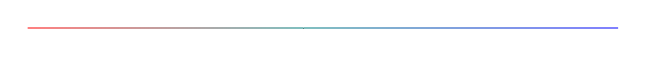
\begin{tikzpicture}
	\fill [left color=red!50, right color=teal!50] (0,0) rectangle (3.5,.01);
	\fill [left color=teal!50, right color=blue!50] (3.5,0) rectangle (7.5,.01);
	\end{tikzpicture}
\vspace{3mm}
\begin{example}
.  Supongamos una función $f=f(r)$, depende solo del módulo de la distancia, 

$$\ r=|\vec r|=\sqrt{x^2+y^2+z^2}$$
\end{example}

Sometemos a $f$ a una simetría de rotaciones $\var \vec r$, ecuación\ref{T15TNtranf}:
$\quad \var f=\var \vec r \cdot \overrightarrow \nabla f=\varepsilon (\hat n\times \vec r)\cdot \overrightarrow \nabla f$

$\cdot \overrightarrow \nabla f=\displaystyle \left( \pdv x , \pdv y, \pdv z\right) \quad r^2=x^2+y^2+z^2 \ \to \begin{cases}
\ \displaystyle  \pdv{x}: \ \ & \displaystyle 2r\pdv{r}{x}=2x \ \to \ \pdv{r}{x}=\dfrac x r \\ \\
\ \displaystyle  \pdv{y}: \ \ & \displaystyle 2r\pdv{r}{y}=2y \ \to \ \pdv{r}{y}=\dfrac y r\\	\\
\ \displaystyle  \pdv{z}: \ \ & \displaystyle 2r\pdv{r}{z}=2z 	 \ \to \ \pdv{r}{z}=\dfrac z r
 \end{cases} $
 
 $\begin{cases}
\ \displaystyle \pdv{f}{x} \ = \ \pdv{f}{r}\pdv{r}{x} \ =\ 	\dfrac x r \pdv{f}{r} \\ \\
\ \displaystyle \pdv{f}{y} \ = \ \pdv{f}{r}\pdv{r}{y} \ =\ 	\dfrac y r \pdv{f}{r} \\ \\
\ \displaystyle \pdv{f}{z} \ = \ \pdv{f}{r}\pdv{r}{z} \ =\ 	\dfrac z r \pdv{f}{r} 
\end{cases}
\ \to \qquad 
\overrightarrow \nabla f=\displaystyle \pdv{f}{r}\ \dfrac 1 r \ (x,y,z) \ = \ \pdv{f}{r}\ \dfrac 1 r \ (x,y,z) \ \vec r $


Así, $\ \boldsymbol{ \var f }=\varepsilon (\hat n\times \vec r)\cdot \overrightarrow \nabla f = \varepsilon (\hat n\times \vec r)\cdot \displaystyle \pdv{f}{r} \dfrac 1 r \vec r=\varepsilon \dfrac 1 r \pdv{f}{r} \ (\hat n \times \vec r) \cdot \vec r=0\, , \ $ ya que $\ (\hat n \times \vec r)\cdot \vec r= \boldsymbol{ 0 }$ 

\vspace{5mm}
\rule{150pt}{0.1pt} 
\vspace{-3mm}

\underline{Inciso 1}: $\ (\hat n \times \vec r)\cdot \vec r=0$  

$\hat n \cdot \vec r=\left( \ [ \hat n \cdot \overrightarrow G]\cdot \vec r \ \right)\cdot \vec r=0\ $ (producto vectorial ec. \ref{T16OFEPV})

Notación tensorial: $\ \ G_i^{jk}\ \ $ elemento de la matriz $\ G_i \ $ en la fila $\ i \ $ y la columna $\ k \ $, por ejemplo, $	\quad G_1^{12}=0,\ G_2^{31}=-1,\ G_3^{21}=1$

$\hat n \times \vec r=
\left( \ [ \hat n \cdot \overrightarrow G]\cdot \vec r \ \right)\cdot \vec r=
(n^i\cdot G_i^{jk}\cdot r_k)\ \cdot  r_j=G_i^{jk}\ r_k \ r_j=0\ $ por tratarse de la contracción de un tensor antisimétrico, $G_i^{jk}$, con uno simétrico, $n^i r_i r_k$. \textcolor{gris}{(Hemos usado el convenio de Einstein, índices repetidos se suman).}

\vspace{-10mm}
\begin{center}
\rule{200pt}{0.1pt}	
\end{center}

\vspace{-3mm}

\underline{Inciso 2, \begin{footnotesize} (de otro modo) \end{footnotesize} }: $\ (\hat n \times \vec r)\cdot \vec r=0$  

$(\vec a \times \vec b)\cdot \vec b =0\, , \ $ ya que $\ \vec a \times \vec b \ \perp \ \vec b \ \to \  (\vec a \times \vec b)\cdot \vec b =0$

\vspace{-8mm}
\begin{flushright}
\rule{200pt}{0.1pt}	
\end{flushright}

\vspace{5mm}

Hemos demostrado que

\begin{equation}
\label{T16ej1}
\text{Si } \ f(r)=\dfrac 1 r \quad \Rightarrow \quad \var f \ = \ 0 \qquad \text{f invariante bajo rotaciones.}	
\end{equation}

Cualquier función que dependa solamente de r (\emph{central}), $\ \boldsymbol{ f=f(r)} \ $, va a ser \textbf{invariante bajo rotaciones}:

$$\var f \ = \ \varepsilon \  \displaystyle \dfrac 1 r \ \pdv{f}{r} \ \cancelto{0}{(\hat n \times \vec r) \cdot \vec r} \ = \ 0$$
 
$$\textbf{\underline{Conclusión ej.1}} \qquad  \subrayado{ \boxed{ \   \boldsymbol{ f=f(r) \ \to \ \var f=0}\, , \ \text{invariante bajo rotaciones infinitesimales} \ } } $$


\vspace{5mm}
\subsection{$\quad f=f(\dot r)$ \textcolor{gris}{$\qquad(\  T=T(\dot r) \ )$}}
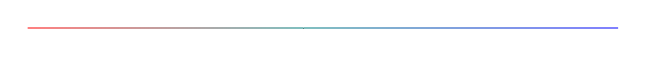
\begin{tikzpicture}
	\fill [left color=red!50, right color=teal!50] (0,0) rectangle (3.5,.01);
	\fill [left color=teal!50, right color=blue!50] (3.5,0) rectangle (7.5,.01);
	\end{tikzpicture}
\vspace{0.5cm}

\begin{example}
-  Supongamos ahora una función $f$ que dependa solo de la velocidad, 

$$ f=f \left(|\dot{\vec r}| \right) = f\left( |\vec v| \right) = f(v)$$
\end{example}

Tenemos definidas las transformaciones infinitesimales de rotación para las posiciones, $\ \var \vec r=\varepsilon \ \hat n \times \vec r\, ,\  $ pero no para las velocidades, $\  \vec v\, . \ $ Como variación y derivada conmutan,

$\var \vec v = \var \dot{\vec r} =\displaystyle  \dot{ \left( {\delta} {\vec r}  \right) } =  \dv{t} \left(  { \var  \vec r }  \right) =  \varepsilon \dv{t} (\hat n \times \vec r) = \varepsilon \left( \cancelto{0}{\dv{\hat n}{t} } \times \vec r + \hat n \times \dot {\vec r} \right)=\varepsilon \ (\hat n \times \dot {\vec r})=\varepsilon (\hat n 	\times \vec v)$

\begin{large}
\begin{myblock}{Transformaciones de velocidades bajo rotaciones infinitesimales: }
\begin{equation}
\label{T16transveloc}
\boldsymbol{ \subrayado{ \ \var \vec v \ = \ \varepsilon \ (\hat n \times \vec v) \ }}
\end{equation}
\end{myblock}
\end{large}


Ahora tendremos $\ \var f=\var \vec v \cdot \displaystyle \left( \pdv{f}{v_x},\pdv{f}{v_y},\pdv{f}{v_z} \right)\, , \ $ pero eso no es el gradiente de $f$.

Como $\ v^2=v_x^2+x_y^2+v_z^2 \ \to \ \displaystyle \pdv{x}\ :\quad 2v\pdv{v}{v_x}=2v_x \ \to \ 
\pdv{v}{v_x}=\dfrac {v_x}{v}$ y análogamente, $\displaystyle \pdv{y},\ \pdv{z}$.


$\displaystyle \left( \pdv{f}{v_x},\pdv{f}{v_y},\pdv{f}{v_z} \right)=\left( \pdv{v}{v_x}\pdv{f}{v},\pdv{v}{v_y}\pdv{f}{v}, \pdv{v}{v_z}\pdv{f}{v} \right) =
\left(\dfrac{v_x}{v},\dfrac{v_y}{v},\dfrac{v_z}{v} \right) \pdv{f}{v}=\dfrac 1 v \pdv{f}{v} \ \left( v_x,v_y,v_z \right) =\dfrac 1 v \pdv{f}{v} \vec v$

Luego, $\ \var f=\var \vec v \cdot \displaystyle \dfrac 1 v \pdv{f}{v} \vec v\, , \ $ sustituyendo $\ \var \vec \, , \ $  ec. \ref{T16transveloc},
$\ \boldsymbol{ \var f} \ = \ \varepsilon \ \displaystyle \dfrac 1 v \ \pdv{f}{v} \ \cancelto{0}{(\hat n \times \vec v) \cdot \vec v} \ = \ \boldsymbol{ 0}$


\vspace{5mm}

$$ \textbf{\underline{Conclusión ej.2}}  \qquad  \quad  \subrayado{ \boxed{ \ 	\boldsymbol{ f=f(v) \ \to \ \var f=0}\, , \ \text{invariante bajo rotaciones infinitesimales} \ }  }$$

\vspace{5mm}
\subsection{$\quad f=f(r, \dot r)$ \textcolor{gris}{$\qquad(\  L=L(r,\dot r) \ )$}}
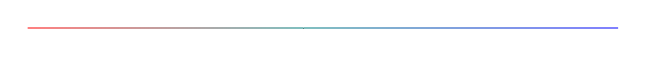
\begin{tikzpicture}
	\fill [left color=red!50, right color=teal!50] (0,0) rectangle (3.5,.01);
	\fill [left color=teal!50, right color=blue!50] (3.5,0) rectangle (7.5,.01);
	\end{tikzpicture}
\vspace{0.5cm}

\begin{example}
.  Ahora suponemos que $f$ depende solamente del modulo de la distancia $r$ y del módulo de la velocidad $v$, 

$$\ f=f(r,v)$$
\end{example}


$\boldsymbol{ \var f}=\var r \cdot \overrightarrow \nabla f + \var v \cdot \displaystyle \left( \pdv{f}{v_x}, \pdv{f}{v_y}, \pdv{f}{v_z} \right) =
\varepsilon \left[  \dfrac 1 r \pdv{f}{r} \cancelto{0}{(\hat n \times \vec r) \cdot \vec r} + \dfrac 1 v \pdv{f}{v} \cancelto{0}{(\hat n \times \vec v)\cdot \vec v} \right]=\boldsymbol{0}$

$$\textbf{\underline{Conclusión ej.3}}  \qquad \quad \subrayado{  \boxed{ \ 	\boldsymbol{ f=f(r,v) \ \to \ \var f=0}\, ,  \ \text{invariante bajo rotaciones infinitesimales} \ }  } $$


\vspace{5mm} Todo lo visto en estos tres ejemplos tiene una repercusión directa en el lagrangiano:

\begin{equation}
\label{T16Lrv}	
\subrayado{
\textbf{Si\ } \  \ \boldsymbol{ L \ = \ \dfrac m 2\ v^2 \ - \ V(r) \ = \  L(r,v) \quad \Rightarrow \quad \var L=0 }
}
\end{equation}

\begin{center} \subrayado{\textbf{ \emph{Los lagrangianos de potencial central son invariantes bajo rotaciones infinitesimales.} } }\end{center}

Si $S$ es la transformación de simetría por rotación, por el teorema de Noether $\ (\var L)_S=0=\displaystyle \dv{K}{t} \ \to \ K=cte=0$ (normalmente se toma cero).



\vspace{10mm}
\section{Teorema de \emph{Noether} para lagrangianos de potencial central}
\vspace{5mm}

\begin{large}
\begin{myblock}{Teorema de Noether para $L\neq L(t)$}
\begin{equation}
\text{Si } \ L\neq L(t) \quad \Rightarrow \quad Q=\sum_{i=1}^n \pdv{L}{\dot q_i} \phi_i-K \, ; \qquad \text{con } \ \phi_i=\dfrac{\var q_i}{\varepsilon}	
\end{equation}	
\end{myblock}
\end{large}

En nuestro caso, $\ \phi=\hat n \times \vec r$, por lo que $\ Q=\displaystyle \pdv{L}{\dot x} \phi_1+\pdv{L}{\dot y} \phi_2+\pdv{L}{\dot z} \phi_3$

$\begin{cases}
\ \phi_1=n_2r_3-n_3r_2 \\ \ \phi_2=n_3r_1-n_1r_3 \\ \ \phi_3=n_1r_2-n_2r_1	
\end{cases} \quad \to  \quad Q=
 \displaystyle \pdv{x} ( n_2r_3-n_3r_2 )  + \displaystyle \pdv{y} ( n_3r_1-n_1r_3) +  \ \displaystyle \pdv{z} (n_1r_2-n_2r_1	) $ 	

$\textcolor{gris}{(r_1=x,\ r_2=y,\ r_3=z) }\, . \ $ Agrupando en $\ n_1, n_2,\ n_3\, : $

\begin{equation}
\label{T16Qcomponentes}
Q=\displaystyle n_1\ \left[ y \  \pdv{L}{\dot z} - z \ \pdv{L}{\dot y} \right] +  
n_2\ \left[ z \  \pdv{L}{\dot x} - x \ \pdv{L}{\dot z} \right]  + n_3\ \left[ x \  \pdv{L}{\dot y} - y \ \pdv{L}{\dot x} \right] 
\end{equation}


Usando la nomenclatura de la formulación de Hamilton, estas derivadas parciales son los \emph{momentos conjugados generalizados} (ec. \ref{T13MomentoCanonicoGeneralizado}) , $\ \displaystyle \pdv{L}{\dot q_i}=p_i\, , \ $ de este modo,

$Q=n_1[yp_z-zp_y]+n_2[zp_x-xp_z]+n_3[xp_y-yp_x]\, , $ donde las expresiones entre corchetes no son más que la expresión del producto vectorial de $vec r \times \vec p\, , \ $

\begin{equation}
\label{T16Q}
	\boxed{ \ \boldsymbol{Q} \ } \ = \hat n \cdot (\vec r \times \vec p) = \ \boxed{ \ \boldsymbol{\hat n \cdot \overrightarrow L } \ } 
\end{equation}


El teorema de Noether, en el caso $L\neq L(t)$ y $K=0$, sabemos que $\displaystyle \dv{Q}{t}=0=\dv{t}(\hat n \cdot \overrightarrow L )$

$\displaystyle \dv{Q}{t}=0=\dv{t}(\hat n \cdot \overrightarrow L )=
\cancelto{0}{\dv{\hat n}{t}} \cdot \overrightarrow L + \hat n \cdot \dot{\overrightarrow  L}= \hat n \cdot \dot{\overrightarrow  L}\, , \ \forall \hat n \ \to \ \subrayado{\boldsymbol{ \boxed{\dot{\overrightarrow  L}=0 \ \ \to \ \ \overrightarrow  L=\overrightarrow {cte}} }}\ $ 

\textbf{Teorema de conservación del momento angular} para lagrangianos independientes del tiempo e invariantes bajo rotaciones.

\vspace{10mm}
\subsection{Usando notación de Relatividad General. Vectores de \emph{Killing}}
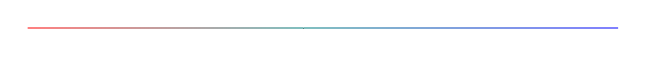
\begin{tikzpicture}
	\fill [left color=red!50, right color=teal!50] (0,0) rectangle (3.5,.01);
	\fill [left color=teal!50, right color=blue!50] (3.5,0) rectangle (7.5,.01);
	\end{tikzpicture}
\vspace{0.5cm}

Volviendo a la ecuación \ref{T16Qcomponentes}, la podemos expresar como
$\ Q=n_1 \ 	\vec \xi_1 \cdot \vec p + n_2 \ 	\vec \xi_2 \cdot \vec p + n_3 \ 	\vec \xi_3 \cdot \vec p \, ,  \ $ dado que $\ \dot Q=0º, , \forall n_1,\ \forall n_2\, , \ \forall n_3 \ \to \ \displaystyle \dv{t} \vec \xi_1 \cdot \vec p=0\, ; \  \dv{t} \vec \xi_2 \cdot \vec p=0\, ; \ \dv{t} \vec \xi_3 \cdot \vec p=0\, . \ $ Para que se cumpla esto ha de ocurrir que

\begin{myalertblock}{Vectores de Killing}
\begin{equation}
\label{T16Vectores Killing}	
\boldsymbol{ \vec \xi_1 \ = \ (0,-z,x)\, ; \quad \vec \xi_2 \ = \ (z,0,-x)\, ; \quad \vec \xi_3 \ = \ (-y,x,0) }
\end{equation}
Vectores de Killing rotacionales de la métrica, aquellas simetrías que dejan invariante la métrica bajo rotaciones.
	
\end{myalertblock}


